\documentclass{beamer}

\title{Preventing Glitches and Short Circuits in\\High-Level Self-Timed Chip Specifications}
\author{Stephen Longfield \and \textbf{Brittany Nkounkou} \and Rajit Manohar \and Ross Tate}
\institute{Cornell University}
\date{}

\setbeamercolor{title}{fg=black}
\setbeamerfont{author}{size=\small}
\setbeamerfont{institute}{size=\small}

\setbeamersize{text margin left=1em, text margin right=1em}
\setbeamertemplate{navigation symbols}

\setbeamercolor{frametitle}{fg=black}

\usepackage{pifont}
\usepackage{mathtools}
\usepackage{stmaryrd}
\usepackage[inference]{semantic}
\usepackage{tikz}
\usetikzlibrary{arrows.meta}
\usetikzlibrary{shapes.arrows}

\newcommand{\noop}{\mathtt{skip}}
\newcommand{\Coloneqq}{\mathrel{::=}}
\newcommand{\p}{\mathop{\parallel}}
\newcommand{\bang}{\mathord{\textrm{<}}}
\newcommand{\query}{\mathord{\textrm{>}}}
\newcommand{\probe}[1]{\bar{#1}}
\newcommand{\probeq}[1]{\hat{#1}}
\newcommand{\true}{\mathbf{true}}
\newcommand{\false}{\mathbf{false}}
\newcommand{\error}{\mathbf{error}}
\newcommand{\idle}{\mathsf{idle}}
\newcommand{\start}{\mathsf{start}}
\newcommand{\use}{\mathsf{use}}
\newcommand{\finish}{\mathsf{finish}}
\newcommand{\holds}[1]{#1\mathsf{~holds}}
\newcommand{\compliant}{\mathbf{compliant}}
\newcommand{\interferant}{\mathbf{interferant}}
\newcommand{\stateto}{\longrightarrow_s}
\newcommand{\traceto}{\longrightarrow_t}
\newcommand{\eff}{\varepsilon}

\definecolor{mygray}{gray}{0.9}
\definecolor{myred}{RGB}{215,25,28}
\definecolor{myorange}{RGB}{253,174,97}
\definecolor{myyellow}{RGB}{255,255,191}
\definecolor{mybabyblue}{RGB}{171,217,233}
\definecolor{myblue}{RGB}{44,123,182}

\begin{document}



\begin{frame}
\begin{center}

\uncover<2>{\begin{tikzpicture}[overlay]
	\node at (0,-6) {\includegraphics[width=\textwidth]{fire}};
\end{tikzpicture}}

\titlepage

\end{center}
\end{frame}



\begin{frame}[t]
\begin{center}

\begin{minipage}[t]{0.49\textwidth}
\begin{center}

\uncover<2->{
{\Large Clocked}

\vspace{1.6em}
\colorbox{mygray}{
\begin{tikzpicture}
	\draw[-, thick] (0.75,2.3) to (1,2.3);
	\draw[-stealth, thick] (2,2.3) to (2.5,2.3);
	\draw[-stealth, thick] (3.5,2.3) to (4,2.3);
	\draw[-, thick] (5,2.3) to (5.25,2.3);
	\draw[-stealth, thick] (2.25,1.25) to (2.25,1.7) to (2.5,1.7);
	\draw[stealth-stealth, thick] (1,1.7) to (0.75,1.7) to  (0.75,1.25) to (3.75,1.25) to (3.75,1.7) to (4,1.7);
	\draw[-, thick] (3,0.75) to (3,1.25);
	\draw[rounded corners, fill=myblue] (1,1.5) rectangle (2,2.5);
	\draw[rounded corners, fill=myorange] (2.5,1.5) rectangle (3.5,2.5);
	\draw[rounded corners, fill=mybabyblue] (4,1.5) rectangle (5,2.5);
	\draw[rounded corners, fill=myyellow] (2,0.5) rectangle (4,1) node[pos=0.5] {Clock};

	\uncover<5-6>{
	\node at (1.5, 2) {\includegraphics[width=.35in]{gears}};
	\node at (3, 2) {\includegraphics[width=.35in]{gears}};
	\node at (4.5, 2) {\includegraphics[width=.35in]{gears}};}
\end{tikzpicture}}}

\end{center}
\end{minipage}
\begin{minipage}[t]{0.49\textwidth}
\begin{center}

\uncover<3->{
\Large Self-Timed

\vspace{2.5em}
\colorbox{mygray}{
\begin{tikzpicture}
	\draw[-, thick] (0.75,0.8) to (1,0.8);
	\draw[-stealth, thick] (2,0.8) to (2.5,0.8);
	\draw[-stealth, thick] (3.5,0.8) to (4,0.8);
	\draw[-, thick] (5,0.8) to (5.25,0.8);
	\draw[-, thick] (0.75,0.5) to (1,0.5);
	\draw[stealth-, thick] (2,0.5) to (2.5,0.5);
	\draw[stealth-, thick] (3.5,0.5) to (4,0.5);
	\draw[-, thick] (5,0.5) to (5.25,0.5);
	\draw[-, thick] (0.75,0.2) to (1,0.2);
	\draw[-stealth, thick] (2,0.2) to (2.5,0.2);
	\draw[-stealth, thick] (3.5,0.2) to (4,0.2);
	\draw[-, thick] (5,0.2) to (5.25,0.2);
	\draw[rounded corners, fill=myblue] (1,0) rectangle(2,1);
	\draw[rounded corners, fill=myorange] (2.5,0) rectangle(3.5,1);
	\draw[rounded corners, fill=mybabyblue] (4,0) rectangle(5,1);

	\uncover<6>{
	\node at (1.5, 0.5) {\includegraphics[width=.15in]{gear}};
	\node at (3, 0.5) {\includegraphics[width=.15in]{gear}};
	\node at (4.5, 0.5) {\includegraphics[width=.15in]{gear}};}
\end{tikzpicture}}}

\end{center}
\end{minipage}

\uncover<11->{\begin{tikzpicture}[overlay]
	\node at (3.1,1.75) {\includegraphics[width=1.5in]{fire}};
\end{tikzpicture}}

\only<4-6>{
\vspace{1.6em}
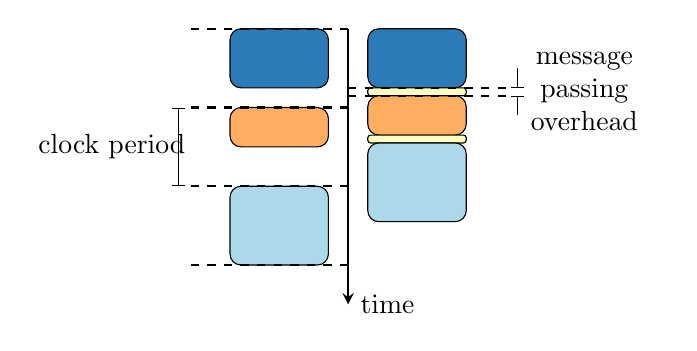
\begin{tikzpicture}
	\draw[-stealth, thick] (0,0) to (0,-3.5);
	\node at (0.5,-3.5) {time};

	\draw[rounded corners, fill=myblue] (-1.5,0) rectangle (-0.25,-0.75);
	\draw[rounded corners, fill=myorange] (-1.5,-1) rectangle (-0.25,-1.5);
	\draw[rounded corners, fill=mybabyblue] (-1.5,-2) rectangle (-0.25,-3);
	\draw[-, thick, dashed] (-2,0) to (0,0);
	\draw[-, thick, dashed] (-2,-1) to (0,-1);
	\draw[-, thick, dashed] (-2,-2) to (0,-2);
	\draw[-, thick, dashed] (-2,-3) to (0,-3);
	\draw[|-|] (-2.15,-1) to (-2.15,-2);
	\node[text width=0.75in, align=center] at (-3,-1.5) {clock period};

	\draw[rounded corners, fill=myblue] (1.5,0) rectangle (0.25,-0.75);
	\draw[rounded corners=1pt, fill=myyellow] (1.5,-0.75) rectangle (0.25,-0.85);
	\draw[rounded corners, fill=myorange] (1.5,-0.85) rectangle (0.25,-1.35);
	\draw[rounded corners=1pt, fill=myyellow] (1.5,-1.35) rectangle (0.25,-1.45);
	\draw[rounded corners, fill=mybabyblue] (1.5,-1.45) rectangle (0.25,-2.45);
	\draw[-, thick, dashed] (0,-0.75) to (2,-0.75);
	\draw[-, thick, dashed] (0,-0.85) to (2,-0.85);
	\draw[-|] (2.15,-0.5) to (2.15,-0.75);
	\draw[|-] (2.15,-0.85) to (2.15,-1.1);
	\node[text width=0.75in, align=center] at (3,-0.8) {message passing overhead};
\end{tikzpicture}}

\only<8->{
\vspace{1em}
\begin{tikzpicture}
	\node at (0,0) {\includegraphics[width=1in]{brain}};
	
	\uncover<9->{
	\node at (-3,1) {\scalebox{-1}[1]{\includegraphics[width=1in]{thought}}};
	\node at (-3,1.1) {sequential};}
	
	\uncover<10->{
	\node at (3,1) {\includegraphics[width=1in]{thought}};
	\node at (3,1.1) {concurrent};}
\end{tikzpicture}}

\end{center}
\end{frame}



\begin{frame}
\begin{center}

\begin{tikzpicture}
	\draw[fill=myyellow] (-1.5,-.5) rectangle (1.5,.5) node[pos=.5] {\Large $P \longrightarrow \invisible{\error}$};
	\node at (-.4,.25) {?};
	\node at (.75,0) {\includegraphics[width=.5in]{fire}};
\end{tikzpicture}

\begin{tikzpicture}[overlay]
	\uncover<2->{
	\node at (2,1.5) {\ding{51}};
	\node at (2,.5) {\ding{55}};}
\end{tikzpicture}

\end{center}
\end{frame}



\begin{frame}
\end{frame}



\begin{frame}[t]
\frametitle{Communicating Hardware Processes (CHP)}
\begin{center}

$\begin{array}{r@{\ }c@{\ }c@{\ }l}
\uncover<2->{\text{Channel} & A} \uncover<21->{& \mathrel{:=} & \langle \bar{A}, \hat{A} \rangle} \\[.75em]
\uncover<3->{\text{Program} & P & \Coloneqq} \uncover<4->{& A!} \uncover<5->{\mid A?} \uncover<28->{\mid A\bang} \uncover<29->{\mid A\query} \\
\uncover<6->{& & & \mid P ; P} \uncover<7->{\mid P \p P} \uncover<8->{\mid *P} \uncover<9->{\mid \noop} \uncover<10->{\mid \ldots}
\end{array}$\\[1em]

\uncover<10->{\hrule\hrule\vspace{1em}}

\only<11-19>{
\uncover<11->{$\only<11>{\invisible{; A!}}P \only<13->{; A!} ; P' \p Q \only<13->{; A?} ; Q'\only<11>{\invisible{; A?}}} \uncover<14->{\longrightarrow \ldots} \uncover<15->{\longrightarrow A! ; P' \p A? ; Q'} \uncover<16->{\longrightarrow P' \p Q'$\\[2em]}

\only<12>{
\begin{tikzpicture}[overlay]
	\draw[-stealth, thick] (-3.9,0.4) to (-3.9,1.1);
	\draw[-stealth, thick] (-2.7,0.4) to (-2.7,1.1);
\end{tikzpicture}}

\uncover<17->{\textbf{ideal:} $A! ; P \p A? ; Q \longrightarrow P \p Q$\\[2em]}

$\uncover<18->{(A! \p A?) \p (A! \p A?)} \uncover<19->{\longrightarrow \invisible{\error}}$

\only<19->{\begin{tikzpicture}[overlay]
\node at (2,0.7) {\includegraphics[width=.5in]{fire}};
\end{tikzpicture}}}

\only<20->{
\uncover<22->{
\colorbox{mygray}{
\begin{minipage}{0.8\textwidth}
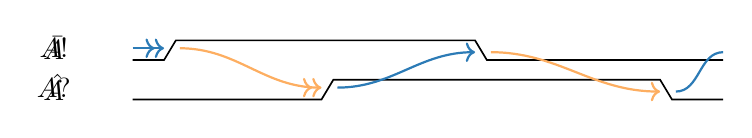
\begin{tikzpicture}
	\node at (0,3.5) {$\bar{A}$};
	\node at (0,3) {$\hat{A}$};
	\draw[-, semithick] (1,3.35) to (1.4,3.35) to (1.55,3.6) to (5.35,3.6) to (5.5,3.35) to (8.5,3.35);
	\draw[-, semithick] (1,2.85) to (3.4,2.85) to (3.55,3.1) to (7.7,3.1) to (7.85,2.85) to (8.5,2.85);
	\uncover<23->{\draw[->>, out=0, in=180, thick, myblue] (1,3.5) to (1.4,3.5);}
	\uncover<24->{\draw[->>, out=0, in=180, thick, myorange] (1.6,3.5) to (3.4,3);}
	\uncover<25->{\draw[->, out=0, in=180, thick, myblue] (3.6,3) to (5.35,3.45);}
	\uncover<26->{\draw[->, out=0, in=180, thick, myorange] (5.55,3.45) to (7.7,2.95);}
	\uncover<27->{\draw[-, out=0, in=180, thick, myblue] (7.9,2.95) to (8.5,3.45);}
	\invisible{
	\node at (0,3.5) {$A!$};
	\node at (0,3) {$A?$};}
\end{tikzpicture}
\end{minipage}}\\[0.5em]}

\uncover<30->{\textbf{ideal:}} \uncover<31->{$A! \p A?} \uncover<32->{\longrightarrow A\bang \p A?} \uncover<33->{\longrightarrow A\bang \p A\query} \uncover<34->{\longrightarrow \noop \p A\query} \uncover<35->{\longrightarrow \noop \p \noop$\\[0.5em]}

\only<36->{
\colorbox{mygray}{
\begin{minipage}{0.8\textwidth}
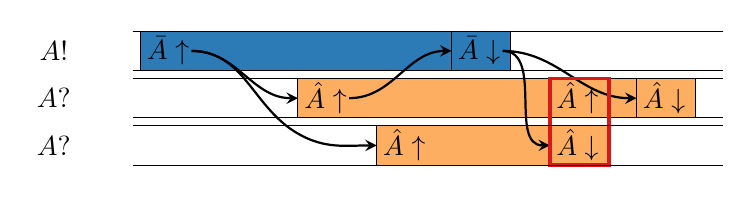
\begin{tikzpicture}
	\node at (0,2.2) {$A!$};
	\node at (0,1.6) {$A?$};
	
	\uncover<37->{
	\draw[fill=myblue] (1.1,1.95) rectangle (5.05,2.45);
	\shade[left color=myblue, right color=mygray] (5,1.95) rectangle (5.8,2.45);
	\node at (1.45,2.2) {$\probe{A} \uparrow$};}
	
	\uncover<38->{
	\draw[-stealth, out=0, in=180, thick] (1.75,2.2) to (3.1,1.6);
	\draw[fill=myorange] (3.1,1.35) rectangle (7.4,1.85);
	\shade[left color=myorange, right color=mygray] (7.35,1.35) rectangle (8.15,1.85);
	\node at (3.45,1.6) {$\probeq{A} \uparrow$};}
	
	\uncover<39->{
	\draw[-stealth, out=0, in=180, thick] (3.75,1.6) to (5.05,2.2);
	\draw[fill=myblue] (5.05,1.95) rectangle (5.8,2.45);
	\node at (5.4,2.2) {$\probe{A} \downarrow$};}
	
	\uncover<40->{
	\draw[-stealth, out=0, in=180, thick] (5.7,2.2) to (7.4,1.6);
	\draw[fill=myorange] (7.4,1.35) rectangle (8.15,1.85);
	\node at (7.75,1.6) {$\probeq{A} \downarrow$};}
	
	\draw[-] (1,2.45) to (8.5,2.45);
	\draw[-] (1,1.95) to (8.5,1.95);
	\draw[-] (1,1.85) to (8.5,1.85);
	\draw[-] (1,1.35) to (8.5,1.35);

	\only<41->{
	\node at (0,1) {$A?$};
	
	\uncover<42->{
	\draw[-, out=0, in=150, thick] (1.75,2.2) to (3.1,1.15);
	\draw[-stealth, out=-30, in=180, thick] (3.1,1.15) to (4.1,1);
	\draw[fill=myorange] (4.1,0.75) rectangle (6.3,1.25);
	\shade[left color=myorange, right color=mygray] (6.25,0.75) rectangle (7.05,1.25);
	\node at (4.45,1) {$\probeq{A} \uparrow$};}
	
	\uncover<43->{
	\draw[-stealth, out=0, in=180, thick] (5.7,2.2) to (6.3,1);
	\draw[fill=myorange] (6.3,0.75) rectangle (7.05,1.25);
	\node at (6.65,1) {$\probeq{A} \downarrow$};}

	\uncover<44->{
	\draw[myred, very thick] (6.3,0.75) rectangle (7.05,1.85);
	\node at (6.65,1.6) {$\probeq{A} \uparrow$};}
	
	\draw[-] (1,1.25) to (8.5,1.25);
	\draw[-] (1,0.75) to (8.5,0.75);}
\end{tikzpicture}
\end{minipage}}\\[0.25em]}

\uncover<44>{\begin{tikzpicture}[overlay]
\node at (2.35,-.9) {\includegraphics[width=.75in]{fire}};
\node at (2.35,-.15) {\textcolor{myred}{\textbf{Short Circuit}}};
\end{tikzpicture}}}

\end{center}
\end{frame}



\begin{frame}
\end{frame}



\begin{frame}[t]
\frametitle{CHP State Semantics}
\begin{center}

\uncover<2->{$\langle P, \sigma \rangle \stateto \langle P', \sigma' \rangle \text{ or } \error$\\[0.5em]}

\uncover<3->{$\sigma$ is a mapping from each $\probe{A}$ and $\probeq{A}$ to a Natural Number\\[1.5em]}

\begin{minipage}[t]{0.49\textwidth}
\begin{center}

\uncover<4->{$\inference{\uncover<5->{\sigma(\probeq{A}) = 0} & \uncover<6->{\sigma(\probe{A}) = n}}{\!\!\!\langle A!, \sigma \rangle \stateto \uncover<7->{\langle A\bang, \sigma[\probe{A} \mapsto n + 1] \rangle}\!\!\!}$\\[1.5em]}

\uncover<8->{$\inference{\uncover<9->{\sigma(\probeq{A}) > 0} & \uncover<10->{\sigma(\probe{A}) = 1}}{\!\!\!\langle A\bang, \sigma \rangle \stateto \uncover<11->{\langle \noop, \sigma[\probe{A} \mapsto 0] \rangle}\!\!\!}$\\[1.5em]}

\uncover<12->{$\inference{\sigma(\probeq{A}) > 0 & \sigma(\probe{A}) > 1}{\!\!\!\langle A\bang, \sigma \rangle \stateto \error\!\!\!}$}

\end{center}
\end{minipage}
\begin{minipage}[t]{0.49\textwidth}
\begin{center}

\uncover<13->{
$\inference{\sigma(\probe{A}) > 0 & \sigma(\probeq{A}) = n}{\!\!\!\langle A?, \sigma \rangle \stateto \langle A\query, \sigma[\probeq{A} \mapsto n + 1] \rangle\!\!\!}$\\[1.5em]

$\inference{\sigma(\probe{A}) = 0 & \sigma(\probeq{A}) = 1}{\!\!\!\langle A\query, \sigma \rangle \stateto \langle \noop, \sigma[\probeq{A} \mapsto 0] \rangle\!\!\!}$\\[1.5em]

$\inference{\sigma(\probe{A}) = 0 & \sigma(\probeq{A}) > 1}{\!\!\!\langle A\query, \sigma \rangle \stateto \error\!\!\!}$}

\end{center}
\end{minipage}\\[1.5em]

\uncover<14>{$\ldots$}

\end{center}
\end{frame}



\begin{frame}[t]
\begin{center}

\begin{tikzpicture}
	\only<1>{
	\draw[fill=myyellow] (-2,-.5) rectangle (2,.5) node[pos=.5] {\Large $\langle P, \sigma_0 \rangle \stateto^* \error$};
	\node at (0.05,.25) {?};}
	
	\only<2->{
	\draw[fill=myyellow] (-3,-.5) rectangle (3,.5) node[pos=.5] {\Large $\langle P \p Q \p R, \sigma_0 \rangle \stateto^* \error$};
	\node at (.9,.25) {?};}
\end{tikzpicture}\\[1em]

\only<3-7>{
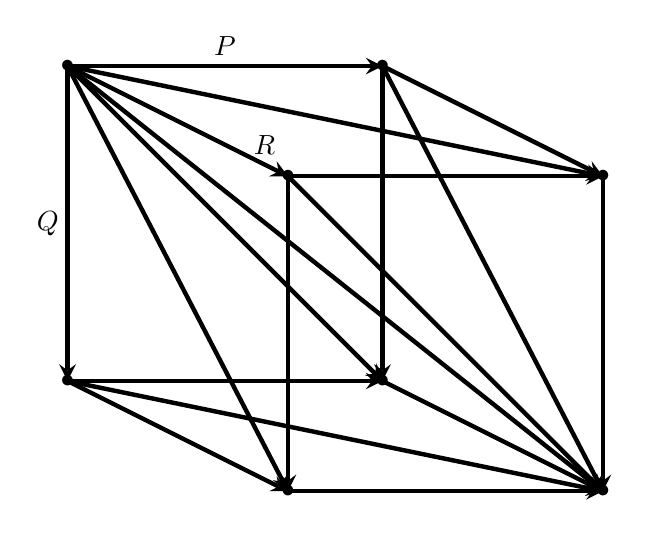
\begin{tikzpicture}
	\draw[-stealth, ultra thick] (0,4) to (4,4);
	\node at (2,4.25) {$P$};
	
	\uncover<4->{\draw[-stealth, ultra thick] (0,4) to (0,0);
	\node at (-0.25,2) {$Q$};}
	
	\uncover<5->{
	\draw[-stealth, ultra thick] (4,4) to (4,0);
	\draw[-stealth, ultra thick] (0,4) to (4,0);
	\draw[-stealth, ultra thick] (0,0) to (4,0);}
	
	\uncover<6->{
	\draw[-stealth, ultra thick] (0,4) to (2.8,2.6);
	\node at (2.5,3) {$R$};}
	
	\uncover<7->{
	\draw[-stealth, ultra thick] (4,4) to (6.8,2.6);
	\draw[-stealth, ultra thick] (0,0) to (2.8,-1.4);
	\draw[-stealth, ultra thick] (4,0) to (6.8,-1.4);
	
	\draw[-stealth, ultra thick] (2.8,2.6) to (6.8,2.6);
	\draw[-stealth, ultra thick] (2.8,2.6) to (2.8,-1.4);
	\draw[-stealth, ultra thick] (6.8,2.6) to (6.8,-1.4);
	\draw[-stealth, ultra thick] (2.8,-1.4) to (6.8,-1.4);
	\draw[-stealth, ultra thick] (2.8,2.6) to (6.8,-1.4);
	
	\draw[-stealth, ultra thick] (0,4) to (6.8,2.6);
	\draw[-stealth, ultra thick] (4,4) to (6.8,-1.4);
	\draw[-stealth, ultra thick] (0,4) to (2.8,-1.4);
	\draw[-stealth, ultra thick] (0,0) to (6.8,-1.4);
	
	\draw[-stealth, ultra thick] (0,4) to (6.8,-1.4);}
	
	\node at (0,4) {$\bullet$};
	\node at (4,4) {$\bullet$};
	
	\uncover<4->{\node at (0,0) {$\bullet$};}
	
	\uncover<5->{\node at (4,0) {$\bullet$};}
	
	\uncover<6->{\node at (2.8,2.6) {$\bullet$};}
	
	\uncover<7->{
	\node at (6.8,2.6) {$\bullet$};
	\node at (2.8,-1.4) {$\bullet$};
	\node at (6.8,-1.4) {$\bullet$};}
\end{tikzpicture}}

\only<9->{
\uncover<12->{
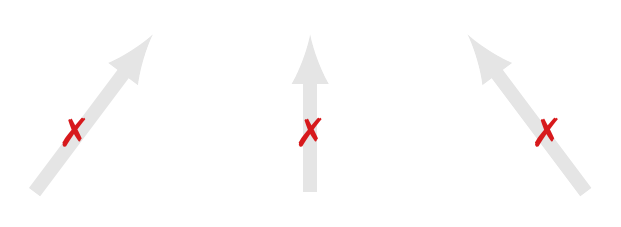
\begin{tikzpicture}
	\draw[-latex, line width=5pt, mygray] (-3.5,0) to (-2,2);
	\draw[-latex, line width=5pt, mygray] (0,0) to (0,2);
	\draw[-latex, line width=5pt, mygray] (3.5,0) to (2,2);
	
	\uncover<14->{
	\node at (-3,.75) {\textcolor{myred}{\Large \ding{55}}};
	\node at (0,.75) {\textcolor{myred}{\Large \ding{55}}};
	\node at (3,.75) {\textcolor{myred}{\Large \ding{55}}};}
\end{tikzpicture}}\\[1em]

\only<9-12>{
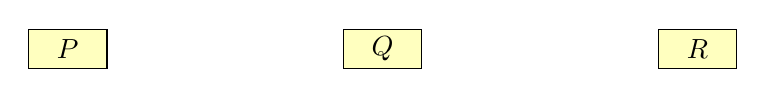
\begin{tikzpicture}
	\draw[fill=myyellow] (-4.5,-.25) rectangle (-3.5,.25) node[pos=.5] {$P$};
	\uncover<10->{\draw[fill=myyellow] (-.5,-.25) rectangle (.5,.25) node[pos=.5] {$Q$};}
	\uncover<11->{\draw[fill=myyellow] (3.5,-.25) rectangle (4.5,.25) node[pos=.5] {$R$};}
\end{tikzpicture}}

\only<13->{
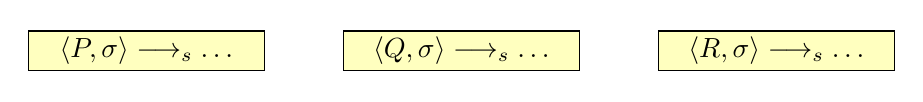
\begin{tikzpicture}
	\draw[fill=myyellow] (-5.5,-.25) rectangle (-2.5,.25) node[pos=.5] {$\langle P, \sigma \rangle \stateto \ldots$};
	\draw[fill=myyellow] (-1.5,-.25) rectangle (1.5,.25) node[pos=.5] {$\langle Q, \sigma \rangle \stateto \ldots$};
	\draw[fill=myyellow] (2.5,-.25) rectangle (5.5,.25) node[pos=.5] {$\langle R, \sigma \rangle \stateto \ldots$};
\end{tikzpicture}}}

\end{center}
\end{frame}



\begin{frame}
\end{frame}



\begin{frame}[t]
\frametitle{CHP Trace Semantics}
\begin{center}

\uncover<2->{$P \xrightarrow{L} P'$\\[0.5em]}

$\begin{array}{r@{\ \Coloneqq\ }l}
\uncover<3->{\text{Label } L} \uncover<4->{& \idle} \uncover<5->{\mid S} \uncover<6->{\mid L \p L} \uncover<7->{\mid \ldots} \\
\uncover<8->{\text{Step } S & M_!^A \mid M_?^A} \\
\uncover<9->{\text{Move } M & \start \mid \use \mid \finish} \\
\end{array}$\\[1em]

\begin{minipage}[t]{0.49\textwidth}
\begin{center}

\uncover<12->{$\inference{\cdot}{\!\!\! A! \xrightarrow{\idle\invisible{^!_!}} A! \!\!\!}$\;\;\;}
\uncover<10->{$\inference{\cdot}{\!\!\! A! \xrightarrow{\start^A_!} A\bang \!\!\!}$\\[1em]}

\uncover<13->{$\inference{\cdot}{\!\!\! A\bang \xrightarrow{\use^A_!} A\bang \!\!\!}$\;\;\;}
\uncover<11->{$\inference{\cdot}{\!\!\! A\bang \xrightarrow{\finish^A_!} \noop \!\!\!}$}

\end{center}
\end{minipage}
\begin{minipage}[t]{0.49\textwidth}
\begin{center}

\uncover<14->{
$\inference{\cdot}{\!\!\! A? \xrightarrow{\idle\invisible{^!_!}} A? \!\!\!}$\;\;\;
$\inference{\cdot}{\!\!\! A? \xrightarrow{\start^A_?} A\query \!\!\!}$\\[1em]

$\inference{\cdot}{\!\!\! A\query \xrightarrow{\use^A_?} A\query \!\!\!}$\;\;\;
$\inference{\cdot}{\!\!\! A\query \xrightarrow{\finish^A_?} \noop \!\!\!}$}

\end{center}
\end{minipage}\\[1.5em]

\uncover<15->{$\inference{P \xrightarrow{L} P' & Q \xrightarrow{K} Q'}{\!\!\! P \p Q \xrightarrow{L \p K} P' \p Q' \!\!\!}$\\[1.5em]}

\uncover<16>{$\ldots$}

\end{center}
\end{frame}



\begin{frame}[t]
\frametitle{CHP Trace Semantics}
\begin{center}

\uncover<2->{$\compliant(L) :=$ traversable in hardware}\\
\uncover<3->{$\interferant(L) :=$ causes a short circuit if traversed}\\[1em]

\begin{minipage}[t]{0.49\textwidth}
\begin{center}

\uncover<4->{$\inference{P \xrightarrow{L} P'\\\compliant(L)\\\neg\interferant(L)}{\!\!\! P \traceto P' \!\!\!}$}

\end{center}
\end{minipage}
\begin{minipage}[t]{0.49\textwidth}
\begin{center}

\uncover<5->{$\inference{P \xrightarrow{L} P'\\\compliant(L)\\\interferant(L) \vee \ldots}{\!\!\! P \traceto \error \!\!\!}$}

\end{center}
\end{minipage}\\[2em]

\uncover<6->{\hrule\hrule\vspace{2em}}

\only<7-9>{
$A\bang \p A\query \xrightarrow{\use^A_! \p \finish^A_?} A\bang \p \noop$\\
\uncover<8>{$\neg\compliant(\use^A_! \p \finish^A_?)$}}

\only<10-13>{
$A\bang \p A\query \xrightarrow{\finish^A_! \p \use^A_?} \noop \p A\query$\\
\uncover<11-12>{$\compliant(\finish^A_! \p \use^A_?)$}\\
\uncover<12>{$\neg\interferant(\finish^A_! \p \use^A_?)$}}

\only<14-17>{
\uncover<14-16>{$A\query \p A\query \xrightarrow{\finish^A_? \p \use^A_?} \noop \p A\query$}\\
\uncover<15-16>{$\compliant(\finish^A_? \p \use^A_?)$}\\
\uncover<16>{$\interferant(\finish^A_? \p \use^A_?)$}}

\end{center}
\end{frame}



\begin{frame}
\end{frame}



\begin{frame}[t]
\only<1>{\frametitle{Semantics Equivalence}}
\only<2->{\frametitle{Inferable Effect System}}
\begin{center}

\begin{tikzpicture}[overlay]
	\node at (4.75,0.25) {\includegraphics[scale=0.1]{aec-badge-pldi}};
\end{tikzpicture}

\begin{tikzpicture}
	\only<1>{\node at (0,0) {$\langle P, \sigma_0 \rangle \stateto^* \error \; \Longleftrightarrow \; P \traceto^* \error$};}
	
	\invisible<1,10>{
	\draw[fill=myyellow] (-1.5,-.5) rectangle (1.5,.5) node[pos=.5] {\Large $P \traceto^* \error$};
	\node at (-.5,.25) {?};}
	
	\only<10>{
	\draw[fill=myyellow] (-2.5,-.5) rectangle (2.5,.5) node[pos=.5] {\Large $P \p Q \p R \traceto^* \error$};
	\node at (.3,.25) {?};}
\end{tikzpicture}\\[1em]

\uncover<3->{$\begin{array}{l@{\;\;\;}c}
P & \eff_P \\
\hline \\
\uncover<4->{A!} & \uncover<5->{A! \xrightarrow{\start^A_!} A\bang \xrightarrow{\finish^A_!} \noop} \\[0.5em]
\uncover<8->{A? & A? \xrightarrow{\start^A_?} A\query \xrightarrow{\finish^A_?} \noop} \\[0.5em]
\uncover<9->{
P ; P & \eff_P \xrightarrow{\idle} \eff_{P'} \\[0.5em]
P \p P' & \eff_P \times \eff_{P'} \\[0.5em]
*P & \eff_P \\[0.5em]
\ldots}
\end{array}$}

\uncover<6>{\begin{tikzpicture}[overlay]
	\node[scale=0.75] at (-1.2,4.7) {$\idle$};
	\draw[-, out=150, in=180, semithick] (-1.3,4.2) to (-1.2,4.5);
	\draw[->, out=0, in=60, semithick] (-1.2,4.5) to (-1.1,4.2);
	\node[scale=0.75] at (0.4,4.7) {$\use^A_!$};
	\draw[-, out=150, in=180, semithick] (0.3,4.2) to (0.4,4.5);
	\draw[->, out=0, in=60, semithick] (0.4,4.5) to (0.5,4.2);
	\node[scale=0.75] at (2.2,4.7) {$\idle$};
	\draw[-, out=150, in=180, semithick] (2.1,4.2) to (2.2,4.5);
	\draw[->, out=0, in=60, semithick] (2.2,4.5) to (2.3,4.2);
\end{tikzpicture}}

\uncover<9->{\begin{tikzpicture}[overlay]
	\node[scale=0.75] at (1.4,1.7) {$\idle$};
	\draw[-, out=0, in=270, semithick] (0.9,1.4) to (1.1,1.5);
	\draw[-, out=90, in=90, semithick] (1.1,1.5) to (0.2,1.5);
	\draw[->, out=270, in=180, semithick] (0.2,1.5) to (0.4,1.4);
\end{tikzpicture}}

\end{center}
\end{frame}



\begin{frame}[t]
\frametitle{Inferable Effect System}
\begin{center}

\invisible{
\begin{tikzpicture}[overlay]
	\node at (4.75,0.25) {\includegraphics[scale=0.1]{aec-badge-pldi}};
\end{tikzpicture}}

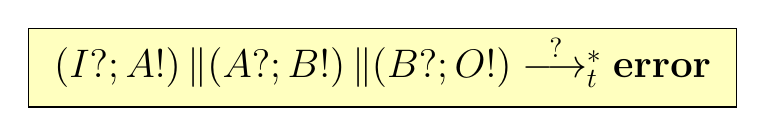
\begin{tikzpicture}
	\draw[fill=myyellow] (-4.5,-.5) rectangle (4.5,.5) node[pos=.5] {\Large $(I?; A!) \p (A?; B!) \p (B?; O!) \traceto^* \error$};
	\node at (2.2,.25) {?};
\end{tikzpicture}\\[1em]

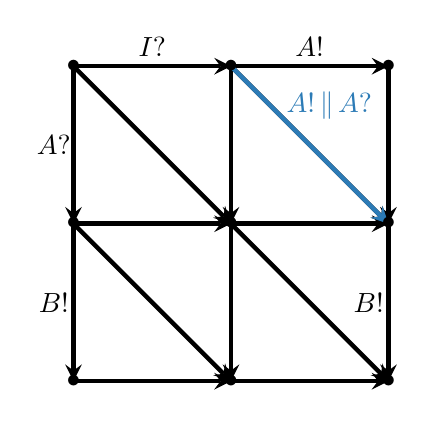
\begin{tikzpicture}
	\uncover<2->{
	\draw[-stealth, ultra thick] (0,4) to (2,4);
	\node at (1,4.25) {$I?$};
	
	\invisible<6->{
	\draw[-stealth, ultra thick] (2,4) to (4,4);
	\node at (3,4.25) {$A!$};}}
	
	\uncover<3->{
	\invisible<6->{
	\draw[-stealth, ultra thick] (0,4) to (0,2);
	\node at (-.25,3) {$A?$};}
	
	\invisible<7->{
	\draw[-stealth, ultra thick] (0,2) to (0,0);
	\node at (-.25,1) {$B!$};}}
	
	\uncover<4->{
	\invisible<7->{
	\draw[-stealth, ultra thick] (0,2) to (2,2);
	\draw[-stealth, ultra thick] (0,0) to (2,0);}
	
	\invisible<6->{
	\draw[-stealth, ultra thick] (2,2) to (4,2);
	\draw[-stealth, ultra thick] (2,0) to (4,0);}
	
	\invisible<6->{
	\draw[-stealth, ultra thick] (2,4) to (2,2);
	\draw[-stealth, ultra thick] (4,4) to (4,2);}
	
	\invisible<7->{\draw[-stealth, ultra thick] (2,2) to (2,0);}
	\draw[-stealth, ultra thick] (4,2) to (4,0);
	\uncover<7>{\node at (3.75,1) {$B!$};}
	
	\invisible<6->{
	\draw[-stealth, ultra thick] (0,4) to (2,2);}
	
	\invisible<5->{\draw[-stealth, ultra thick] (2,4) to (4,2);}
	\uncover<5->{\draw[-stealth, ultra thick, myblue] (2,4) to (4,2);}
	\uncover<5->{\node at (3.25,3.5) {\textcolor{myblue}{$A! \p A?$}};}
	
	\invisible<7->{\draw[-stealth, ultra thick] (0,2) to (2,0);}
	
	\invisible<6->{
	\draw[-stealth, ultra thick] (2,2) to (4,0);}}
	
	\uncover<2->{
	\node at (0,4) {$\bullet$};
	\node at (2,4) {$\bullet$};
	\invisible<6->{\node at (4,4) {$\bullet$};}}
	
	\uncover<3->{
	\invisible<7->{
	\node at (0,2) {$\bullet$};
	\node at (0,0) {$\bullet$};}}
	
	\uncover<4->{
	\invisible<7->{
	\node at (2,2) {$\bullet$};
	\node at (2,0) {$\bullet$};}
	
	\node at (4,2) {$\bullet$};
	\node at (4,0) {$\bullet$};}
\end{tikzpicture}

\end{center}
\end{frame}



\begin{frame}[t]
\frametitle{Inferable Effect System}
\begin{center}

\invisible{
\begin{tikzpicture}[overlay]
	\node at (4.75,0.25) {\includegraphics[scale=0.1]{aec-badge-pldi}};
\end{tikzpicture}}

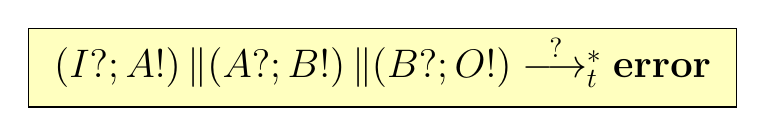
\begin{tikzpicture}
	\draw[fill=myyellow] (-4.5,-.5) rectangle (4.5,.5) node[pos=.5] {\Large $(I?; A!) \p (A?; B!) \p (B?; O!) \traceto^* \error$};
	\node at (2.2,.25) {?};
\end{tikzpicture}\\[1em]

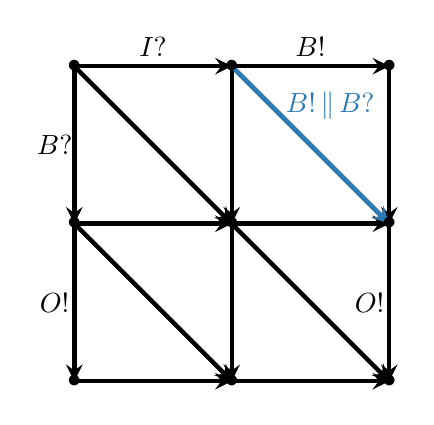
\begin{tikzpicture}
	\draw[-stealth, ultra thick] (0,4) to (2,4);
	\node at (1,4.25) {$I?$};
	
	\invisible<5->{
	\draw[-stealth, ultra thick] (2,4) to (4,4);
	\node at (3,4.25) {$B!$};}
	
	\uncover<2->{
	\invisible<5->{
	\draw[-stealth, ultra thick] (0,4) to (0,2);
	\node at (-.25,3) {$B?$};}
	
	\invisible<6->{
	\draw[-stealth, ultra thick] (0,2) to (0,0);
	\node at (-.25,1) {$O!$};}}
	
	\uncover<3->{
	\invisible<6->{
	\draw[-stealth, ultra thick] (0,2) to (2,2);
	\draw[-stealth, ultra thick] (0,0) to (2,0);}
	
	\invisible<5->{
	\draw[-stealth, ultra thick] (2,2) to (4,2);
	\draw[-stealth, ultra thick] (2,0) to (4,0);}
	
	\invisible<5->{
	\draw[-stealth, ultra thick] (2,4) to (2,2);
	\draw[-stealth, ultra thick] (4,4) to (4,2);}
	
	\invisible<6->{\draw[-stealth, ultra thick] (2,2) to (2,0);}
	\draw[-stealth, ultra thick] (4,2) to (4,0);
	\uncover<6>{\node at (3.75,1) {$O!$};}
	
	\invisible<5->{
	\draw[-stealth, ultra thick] (0,4) to (2,2);}
	
	\invisible<4->{\draw[-stealth, ultra thick] (2,4) to (4,2);}
	\uncover<4->{\draw[-stealth, ultra thick, myblue] (2,4) to (4,2);}
	\uncover<4->{\node at (3.25,3.5) {\textcolor{myblue}{$B! \p B?$}};}
	
	\invisible<6->{\draw[-stealth, ultra thick] (0,2) to (2,0);}
	
	\invisible<5->{
	\draw[-stealth, ultra thick] (2,2) to (4,0);}}
	
	\node at (0,4) {$\bullet$};
	\node at (2,4) {$\bullet$};
	\invisible<5->{\node at (4,4) {$\bullet$};}
	
	\uncover<2->{
	\invisible<6->{
	\node at (0,2) {$\bullet$};
	\node at (0,0) {$\bullet$};}}
	
	\uncover<3->{
	\invisible<6->{
	\node at (2,2) {$\bullet$};
	\node at (2,0) {$\bullet$};}
	
	\node at (4,2) {$\bullet$};
	\node at (4,0) {$\bullet$};}
\end{tikzpicture}

\end{center}
\end{frame}



\begin{frame}[t]
\frametitle{Inferable Effect System}
\begin{center}

\invisible{
\begin{tikzpicture}[overlay]
	\node at (4.75,0.25) {\includegraphics[scale=0.1]{aec-badge-pldi}};
\end{tikzpicture}}

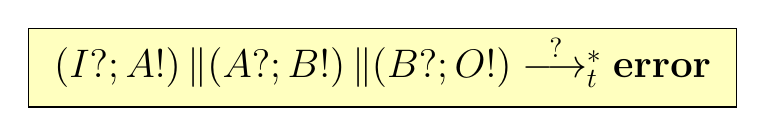
\begin{tikzpicture}
	\draw[fill=myyellow] (-4.5,-.5) rectangle (4.5,.5) node[pos=.5] {\Large $(I?; A!) \p (A?; B!) \p (B?; O!) \traceto^* \error$};
	\node at (2.2,.25) {?};
\end{tikzpicture}\\[1em]

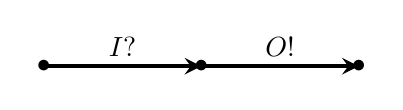
\begin{tikzpicture}
	\draw[-stealth, ultra thick] (0,4) to (2,4);
	\node at (1,4.25) {$I?$};
	
	\draw[-stealth, ultra thick] (2,4) to (4,4);
	\node at (3,4.25) {$O!$};

	\node at (0,4) {$\bullet$};
	\node at (2,4) {$\bullet$};
	\node at (4,4) {$\bullet$};
\end{tikzpicture}\\[1em]

\uncover<2->{3 states vs. 27 states}

\end{center}
\end{frame}



\begin{frame}
\end{frame}



\begin{frame}
\frametitle{Performance Evaluation}
\begin{center}
\uncover<2-6>{\includegraphics[width=\textwidth]{results}}

\begin{tikzpicture}[overlay]
	\uncover<3>{
	\draw[line width=3pt] (-4.47,1.6) rectangle (-3.04,5.1);
	\draw[line width=3pt] (1.65,1.6) rectangle (3.1,5.1);}
	
	\uncover<4>{
	\draw[line width=3pt] (-1.82,1.6) rectangle (-.39,5.1);
	\draw[line width=3pt] (4.3,1.6) rectangle (5.75,5.1);}
	
	\uncover<5>{
	\draw[line width=3pt] (-4.95,1.6) rectangle (-4.37,5.1);
	\draw[line width=3pt] (1.25,1.6) rectangle (1.81,5.1);}
\end{tikzpicture}

\end{center}
\end{frame}



\begin{frame}
\end{frame}



\begin{frame}
\frametitle{Conclusion}
\begin{center}
\begin{minipage}{.9\textwidth}

\Large

\uncover<2->{\makebox[0pt][l]{$\square$}\raisebox{.15ex}{\hspace{0.1em}$\checkmark$} CHP Trace Semantics}

\uncover<3->{\makebox[0pt][l]{$\square$}\raisebox{.15ex}{\hspace{0.1em}$\checkmark$} Inferable Effect System}\\[1em]

\uncover<4->{\makebox[0pt][l]{$\square$}\raisebox{.15ex}{\hspace{0.1em}\invisible{$\checkmark$}} include data in semantics proof of equivalence}

\uncover<5->{\makebox[0pt][l]{$\square$}\raisebox{.15ex}{\hspace{0.1em}\invisible{$\checkmark$}} verify tool}

\uncover<6->{\makebox[0pt][l]{$\square$}\raisebox{.15ex}{\hspace{0.1em}\invisible{$\checkmark$}} explore other aspects of CHP design process}

\end{minipage}
\end{center}
\end{frame}


\begin{frame}
\begin{center}

\begin{tikzpicture}[overlay]
	\node at (0,-4.25) {\includegraphics[width=\textwidth]{fire}};
\end{tikzpicture}

\Large Thank you! Questions?

\end{center}
\end{frame}



\end{document}